\documentclass[a4paper,11pt, colorinlistoftodos]{book}
%\documentclass[a4paper,twoside,11pt,titlepage]{book}
\usepackage{listings}
\usepackage[utf8]{inputenc}
\usepackage[spanish, es-tabla]{babel}
\usepackage{eurosym}
%\usepackage{cite}

\usepackage[loadshadowlibrary]{todonotes}
\usepackage{float, subcaption}

\usepackage{colortbl}
\usepackage{multirow}
\usepackage{multicol}
\definecolor{M1}{RGB}{255,199,2}

\usepackage{amsmath}
\usepackage{dirtytalk}
\usepackage{xcolor}
\usepackage{tikz}
\usepackage{makecell}

\newcommand{\code}{\lstinline}

\usepackage{csquotes}
\usepackage{microtype}
\usepackage[backend=biber, defernumbers=true, citestyle=numeric-comp, bibstyle=ieee, sorting=none]{biblatex}

\DeclareBibliographyCategory{cited}
\AtEveryCitekey{\addtocategory{cited}{\thefield{entrykey}}}
% Configurando BibLaTeX
\DefineBibliographyStrings{spanish}{
  url = {URL},
  andothers={et ~al\adddot}
}

\addbibresource{bibliografia/bibliografia.bib}

\setlength{\parindent}{0pt}

\definecolor{ugr_yellow}{rgb}{1.0, 0.78, 0}

\newcommand{\addref}[2][1=]{\todo[shadow, color=black!40, caption={Pendiente Referencia: #1}]{#2}}
\newcommand{\towrite}[2][1=]{\todo[inline, shadow, color=gray!40, caption={A escribir: #1}]{En proceso: #2}}
\newcommand{\corrected}[2][1=]{\todo[inline, shadow, color=blue!40, caption={Propuesta: #1}]{#2}}
\newcommand{\changed}[2][1=]{\todo[shadow, color=yellow!40, caption={Cambios: #1}]{#2}}

\newcommand{\Enrique}[2][1=]{\todo[inline, shadow, color=red!40, caption={Enrique: #1}]{#2}}
\newcommand{\EnriqueL}[2][1=]{\todo[shadow, color=red!40, caption={Enrique: #1}]{#2}}
\newcommand{\Mesejo}[2][1=]{\todo[inline, shadow, color=orange!40, caption={Pablo: #1}]{#2}}
\newcommand{\MesejoL}[2][1=]{\todo[shadow, color=orange!40, caption={Pablo: #1}]{#2}}
\newcommand{\Brian}[2][1=]{\todo[inline, shadow, color=yellow!40, caption={Brian: #1}]{#2}}

%\usepackage[style=list, number=none]{glossary} %
%\usepackage{titlesec}
%\usepackage{pailatino}

\decimalpoint
\usepackage{dcolumn}
\newcolumntype{.}{D{.}{\esperiod}{-1}}
\makeatletter
\addto\shorthandsspanish{\let\esperiod\es@period@code}
\makeatother


%\usepackage[chapter]{algorithm}
\RequirePackage{verbatim}
%\RequirePackage[Glenn]{fncychap}
\usepackage{fancyhdr}
\usepackage{graphicx}
\usepackage{afterpage}

\usepackage{longtable}

\usepackage[pdfborder={000}, hidelinks]{hyperref} %referencia

% ********************************************************************
% Re-usable information
% ********************************************************************
\newcommand{\myTitle}{Metrología Monocular en Entornos No Controlados}
\newcommand{\mySubTitle}{}
\newcommand{\myTitleENG}{Single View Metrology in the Wild}
\newcommand{\mySubTitleENG}{}
\newcommand{\myDegree}{Máster en Ciencia de Datos e Ingeniería de Computadores}
\newcommand{\myName}{Brian Sena Simons}
\newcommand{\myProf}{Pablo Mesejo Santiago}
\newcommand{\myOtherProf}{Enrique Bermejo Nievas}
%\newcommand{\mySupervisor}{Put name here}
\newcommand{\myFaculty}{Escuela Técnica Superior de Ingenierías Informática y de
Telecomunicación}
\newcommand{\myFacultyShort}{E.T.S. de Ingenierías Informática y de
Telecomunicación}
\newcommand{\myDepartment}{Departamento de Ciencias de la Computación e Inteligencia Artificial }
\newcommand{\myUni}{\protect{Universidad de Granada}}
\newcommand{\myLocation}{Granada}
\newcommand{\myTime}{\today}
\newcommand{\myVersion}{Version 0.1}


\hypersetup{
pdfauthor = {\myName (briansenas@correo.ugr.es)},
pdftitle = {\myTitle},
pdfsubject = {},
% NOTE: update this once we finish
pdfkeywords = {palabra_clave1, palabra_clave2, palabra_clave3, ...},
pdfcreator = {LaTeX con el paquete pdflatex},
pdfproducer = {pdflatex}
}

%\hyphenation{}


%\usepackage{doxygen/doxygen}
%\usepackage{pdfpages}
\usepackage{url}
\usepackage{colortbl,longtable}
\usepackage[stable]{footmisc}
%\usepackage{index}

%\makeindex
%\usepackage[style=long, cols=2,border=plain,toc=true,number=none]{glossary}
%\makeglossary

% Definición de comandos que me son tiles:
%\renewcommand{\indexname}{Índice alfabético}
%\renewcommand{\glossaryname}{Glosario}

\pagestyle{fancy}
\fancyhf{}
\fancyhead[LO]{\leftmark}
\fancyhead[RE]{\rightmark}
\fancyhead[RO,LE]{\textbf{\thepage}}
\renewcommand{\chaptermark}[1]{\markboth{\textbf{#1}}{}}
\renewcommand{\sectionmark}[1]{\markright{\textbf{\thesection. #1}}}

\setlength{\headheight}{1.5\headheight}

\newcommand{\HRule}{\rule{\linewidth}{0.5mm}}
%Definimos los tipos teorema, ejemplo y definición podremos usar estos tipos
%simplemente poniendo \begin{teorema} \end{teorema} ...
\newtheorem{teorema}{Teorema}[chapter]
\newtheorem{ejemplo}{Ejemplo}[chapter]
\newtheorem{definicion}{Definición}[chapter]

\definecolor{gray97}{gray}{.97}
\definecolor{gray75}{gray}{.75}
\definecolor{gray45}{gray}{.45}
\definecolor{gray30}{gray}{.94}

\lstset{ frame=Ltb,
     framerule=0.5pt,
     aboveskip=0.5cm,
     framextopmargin=3pt,
     framexbottommargin=3pt,
     framexleftmargin=0.1cm,
     framesep=0pt,
     rulesep=.4pt,
     backgroundcolor=\color{gray97},
     rulesepcolor=\color{black},
     %
     stringstyle=\ttfamily,
     showstringspaces = false,
     basicstyle=\normalsize\ttfamily,
     commentstyle=\color{gray45},
     keywordstyle=\bfseries,
     %
     numbers=left,
     numbersep=6pt,
     numberstyle=\tiny,
     numberfirstline = false,
     breaklines=true,
   }
 
% minimizar fragmentado de listados
\lstnewenvironment{listing}[1][]
   {\lstset{#1}\pagebreak[0]}{\pagebreak[0]}

\lstdefinestyle{CodigoC}
   {
	basicstyle=\scriptsize,
	frame=single,
	language=C,
	numbers=left
   }
\lstdefinestyle{CodigoC++}
   {
	basicstyle=\small,
	frame=single,
	backgroundcolor=\color{gray30},
	language=C++,
	numbers=left
   }

 
\lstdefinestyle{Consola}
   {basicstyle=\scriptsize\bf\ttfamily,
    backgroundcolor=\color{gray30},
    frame=single,
    numbers=none
   }


\newcommand{\bigrule}{\titlerule[0.5mm]}


%Para conseguir que en las páginas en blanco no ponga cabecerass
\makeatletter
\def\clearpage{%
  \ifvmode
    \ifnum \@dbltopnum =\m@ne
      \ifdim \pagetotal <\topskip
        \hbox{}
      \fi
    \fi
  \fi
  \newpage
  \thispagestyle{empty}
  \write\m@ne{}
  \vbox{}
  \penalty -\@Mi
}
\makeatother

\usepackage{pdfpages}


% % Temporarly
% \usepackage{fancyhdr}
% \pagestyle{fancyplain}
% \fancyhead{}
% \lfoot{\scriptsize\LaTeX}
% \cfoot{\hyperlink{listoftodos}{ToDoList} || \hyperlink{tableofcontents}{TableOfContents}}
% \rfoot{\small\thepage}

\begin{document}
\begin{titlepage}
 
\newlength{\centeroffset}
\setlength{\centeroffset}{-0.5\oddsidemargin}
\addtolength{\centeroffset}{0.5\evensidemargin}

\thispagestyle{empty}

\noindent\hspace*{\centeroffset}\begin{minipage}{\textwidth}

\centering

\includegraphics[width=0.9\textwidth]{imagenes/logo_ugr.jpg}\\[1.4cm]

\textsc{ \Large TRABAJO FIN DE MÁSTER\\[0.2cm]}
\textsc{ CIENCIA DE DATOS E INGENIERÍA DE COMPUTADORES}\\[1cm]
% Upper part of the page
% 
% Title
{\LARGE\bfseries \myTitle\\
}
\noindent\rule[-1ex]{\textwidth}{3pt}\\[3.5ex]
{\large\bfseries \mySubTitle}
\end{minipage}

\vspace{2.0cm}
\noindent\hspace*{\centeroffset}\begin{minipage}{\textwidth}
\centering

\textbf{Autor}\\ {\myName}\\[2.5ex]
\textbf{Directores}\\
{\myProf\\
\myOtherProf}\\[2cm]

\includegraphics[width=0.3\textwidth]{imagenes/etsiit_logo.png}\\[0.1cm]
\textsc{\myFaculty}\\
\textsc{---}\\
Granada, Septiembre de 2025
\end{minipage}
%\addtolength{\textwidth}{\centeroffset}
%\vspace{\stretch{2}}
\end{titlepage}

\chapter*{}
%\thispagestyle{empty}
%\cleardoublepage

%\thispagestyle{empty}

% \begin{titlepage}
 
\setlength{\centeroffset}{-0.5\oddsidemargin}
\addtolength{\centeroffset}{0.5\evensidemargin}

\thispagestyle{empty}

\noindent\hspace*{\centeroffset}\begin{minipage}{\textwidth}

\centering
%
\includegraphics[width=0.9\textwidth]{imagenes/logo_ugr.jpg}\\[1.4cm]

%\textsc{ \Large PROYECTO FIN DE CARRERA\\[0.2cm]}
%\textsc{ INGENIERÍA EN INFORMÁTICA}\\[1cm]
% Upper part of the page
% 

 \vspace{3.3cm}

%si el proyecto tiene logo poner aquí
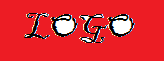
\includegraphics{imagenes/logo.png} 
 \vspace{0.5cm}

% Title

{\Huge\bfseries \myTitle\\
}
\noindent\rule[-1ex]{\textwidth}{3pt}\\[3.5ex]
{\large\bfseries \mySubTitle\\[4cm]}
\end{minipage}

\vspace{2.5cm}
\noindent\hspace*{\centeroffset}\begin{minipage}{\textwidth}
\centering

\textbf{Autor}\\ {\myName}\\[2.5ex]
\textbf{Directores}\\
{\myProf\\
\myOtherProf}\\[2cm]
%
\includegraphics[width=0.15\textwidth]{imagenes/tstc.png}\\[0.1cm]
%\textsc{\myDepartment}\\
%\textsc{---}\\
%Granada, mes de 201
\end{minipage}
%\addtolength{\textwidth}{\centeroffset}
\vspace{\stretch{2}}

 
\end{titlepage}



%\cleardoublepage
\thispagestyle{empty}

\begin{center}
{\large\bfseries \myTitle}\\
\end{center}
\begin{center}
\myName\\
\end{center}

%\vspace{0.7cm}
\noindent{\textbf{Palabras clave}: 
}\\

\noindent{\textbf{Resumen}}\\
\cleardoublepage


\thispagestyle{empty}


\begin{center}
{\large\bfseries \myTitleENG}\\
\end{center}
\begin{center}
\myName \\
\end{center}

%\vspace{0.7cm}
\noindent{\textbf{Keywords}: 
}\\

%\vspace{0.7cm}
\noindent{\textbf{Abstract}}\\

\chapter*{}
\thispagestyle{empty}

\noindent\rule[-1ex]{\textwidth}{2pt}\\[4.5ex]

Yo, \textbf{\myName}, alumno de la titulación Máster en Ciencia de Datos e Ingeniería de Computadores
de la \textbf{\myFaculty}, 
con Pasaporte NX4L843F5, autorizo la ubicación de la siguiente copia de mi 
Trabajo Fin de Máster en la biblioteca del centro para que pueda ser
consultada por las personas que lo deseen.

\vspace{6cm}

\noindent Fdo: \myName

\vspace{2cm}

\begin{flushright}
Granada a \today.
\end{flushright}


\chapter*{}
\thispagestyle{empty}

\noindent\rule[-1ex]{\textwidth}{2pt}\\[4.5ex]

D. \textbf{\myProf}, Profesor del \myDepartment de la Universidad de Granada.

\vspace{0.5cm}

D. \textbf{\myOtherProf}, Profesor del \myDepartment de la Universidad de Granada.


\vspace{0.5cm}

\textbf{Informan:}

\vspace{0.5cm}

Que el presente trabajo, titulado \textit{\textbf{\myTitle}}
ha sido realizado bajo su supervisión por \textbf{\myName}, y autorizamos la defensa de dicho trabajo ante el tribunal
que corresponda.

\vspace{0.5cm}

Y para que conste, expiden y firman el presente informe en Granada a \today.

\vspace{1cm}

\textbf{Los directores:}

\vspace{5cm}

\noindent \textbf{\myProf \ \ \ \ \ \myOtherProf}

\chapter*{Agradecimientos}

\thispagestyle{empty}
       \vspace{1cm}


Primeramente, me gustaría agradecer a mis tutores, Enrique Bermejo y Pablo Mesejo,
por darme la oportunidad de desarrollar este proyecto con ellos. 
Agradezco la paciencia infinita y comprensión a la hora de resolver mis dudas. 
Segundo, agradezco a la propia Universidad de Granada por haberme dado la oportunidad 
de continuar mis estudios universitarios en tan distinguida casa de estudios. 
\\

\frontmatter
\mainmatter

\hypertarget{listoftodos}{}
%\listoftodos[Anotaciones y Cambios]

\tableofcontents
\listoffigures
\listoftables
\setlength{\parskip}{5pt}

\chapter{Introducción}
\section{Definición del Problema}   
\section{Motivación}
\section{Objetivos}
\section{Planificación del proyecto}

%
\chapter{Fundamentos Teóricos}
\section{Modelado de cámara}
La formación de imágenes en sistemas de visión por computadora se basa en la proyección perspectiva, 
un modelo geométrico que describe cómo los puntos del espacio tridimensional (3D), habitualmente denominado
las coordenadas del mundo, se proyectan sobre un plano bidimensional (2D), el plano de la imagen. 
En la Figura~\ref{fig:PinHole} se observa el modelo fundamental, de cámara estenopeica, 
que idealiza la cámara como un sistema sin lentes donde los rayos de luz pasan por un solo punto. 
Un punto perteneciente al espacio 3D, $P=(X,Y,Z)$, se proyecta
sobre el plano de imagen utilizando las relaciones definidas en la Ecuación~\ref{eq:2DProyection},
tras aplicar la semejanza entre triángulos~\cite{Hartley2004,VisionBookMIT}. 
\begin{equation}\label{eq:2DProyection}
    x=f\cdot\frac{X}{Z}, \; y=f\cdot\frac{Y}{Z}
\end{equation}

\begin{figure}[htp]
\begin{center}
    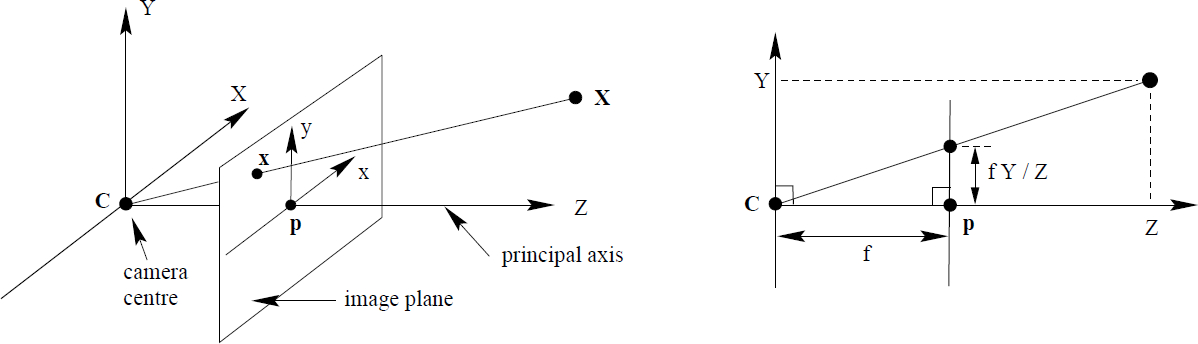
\includegraphics[width=0.7\textwidth]{imagenes/chapter2/pinhole-model}
\end{center}
\caption{
    Se observa la geometría subyaciente del modelo de cámara estenopeico sacada de~\cite{Hartley2004}.
    La distancia entre el punto principal, P, y el centro de la cámara se denomina distancia focal, f, y
    nos permite obtener la relación entre la coordenadas del plano de imagen y del punto en las coordenadas 
    del mundo utilizando trigonometría.
}
\label{fig:PinHole}
\end{figure}

La Ecuación~\ref{eq:2DProyection} define la proyección de perspectiva, donde objetos distantes aparentan más pequeños,
con un escalado inverso a su distancia en el eje Z. Este modelo también se aplica a la visión humana.
Esta transformación se puede expresar de forma matricial mediante coordenadas homogéneas. Si $P=(X,Y,Z,1)^T$ y $p=(x, y, 1)^T$, 
la proyección se puede expresar acorde a la Ecuación~\ref{eq:ProyectionFormula}.

\begin{equation}\label{eq:ProyectionFormula}
    s\begin{bmatrix}x\\y\\1\end{bmatrix} = K\cdot\left[R|t\right]\cdot\begin{bmatrix}X\\Y\\Z\\1\end{bmatrix}
\end{equation}

Donde $K$ es la matriz intrínseca de la cámara, que contiene los parámetros internos como la distancia focal y el 
punto principal, véase la Ecuación~\ref{eq:KMatrix}. $[R|t]$ es la concatenación de la matriz de rotación R y
el vector de traslación t, que definen la posición y orientación de la cámara respecto al eje del mundo (parámetros extrínsecos).
Por último, $s$ sería un factor de escala. Este modelo permite modelar coordenadas 3D del mundo a píxeles de la imagen, véase la 
Figura~\ref{fig:WorldToImageCoordinates}. 

\begin{figure}[htp]
\begin{center}
    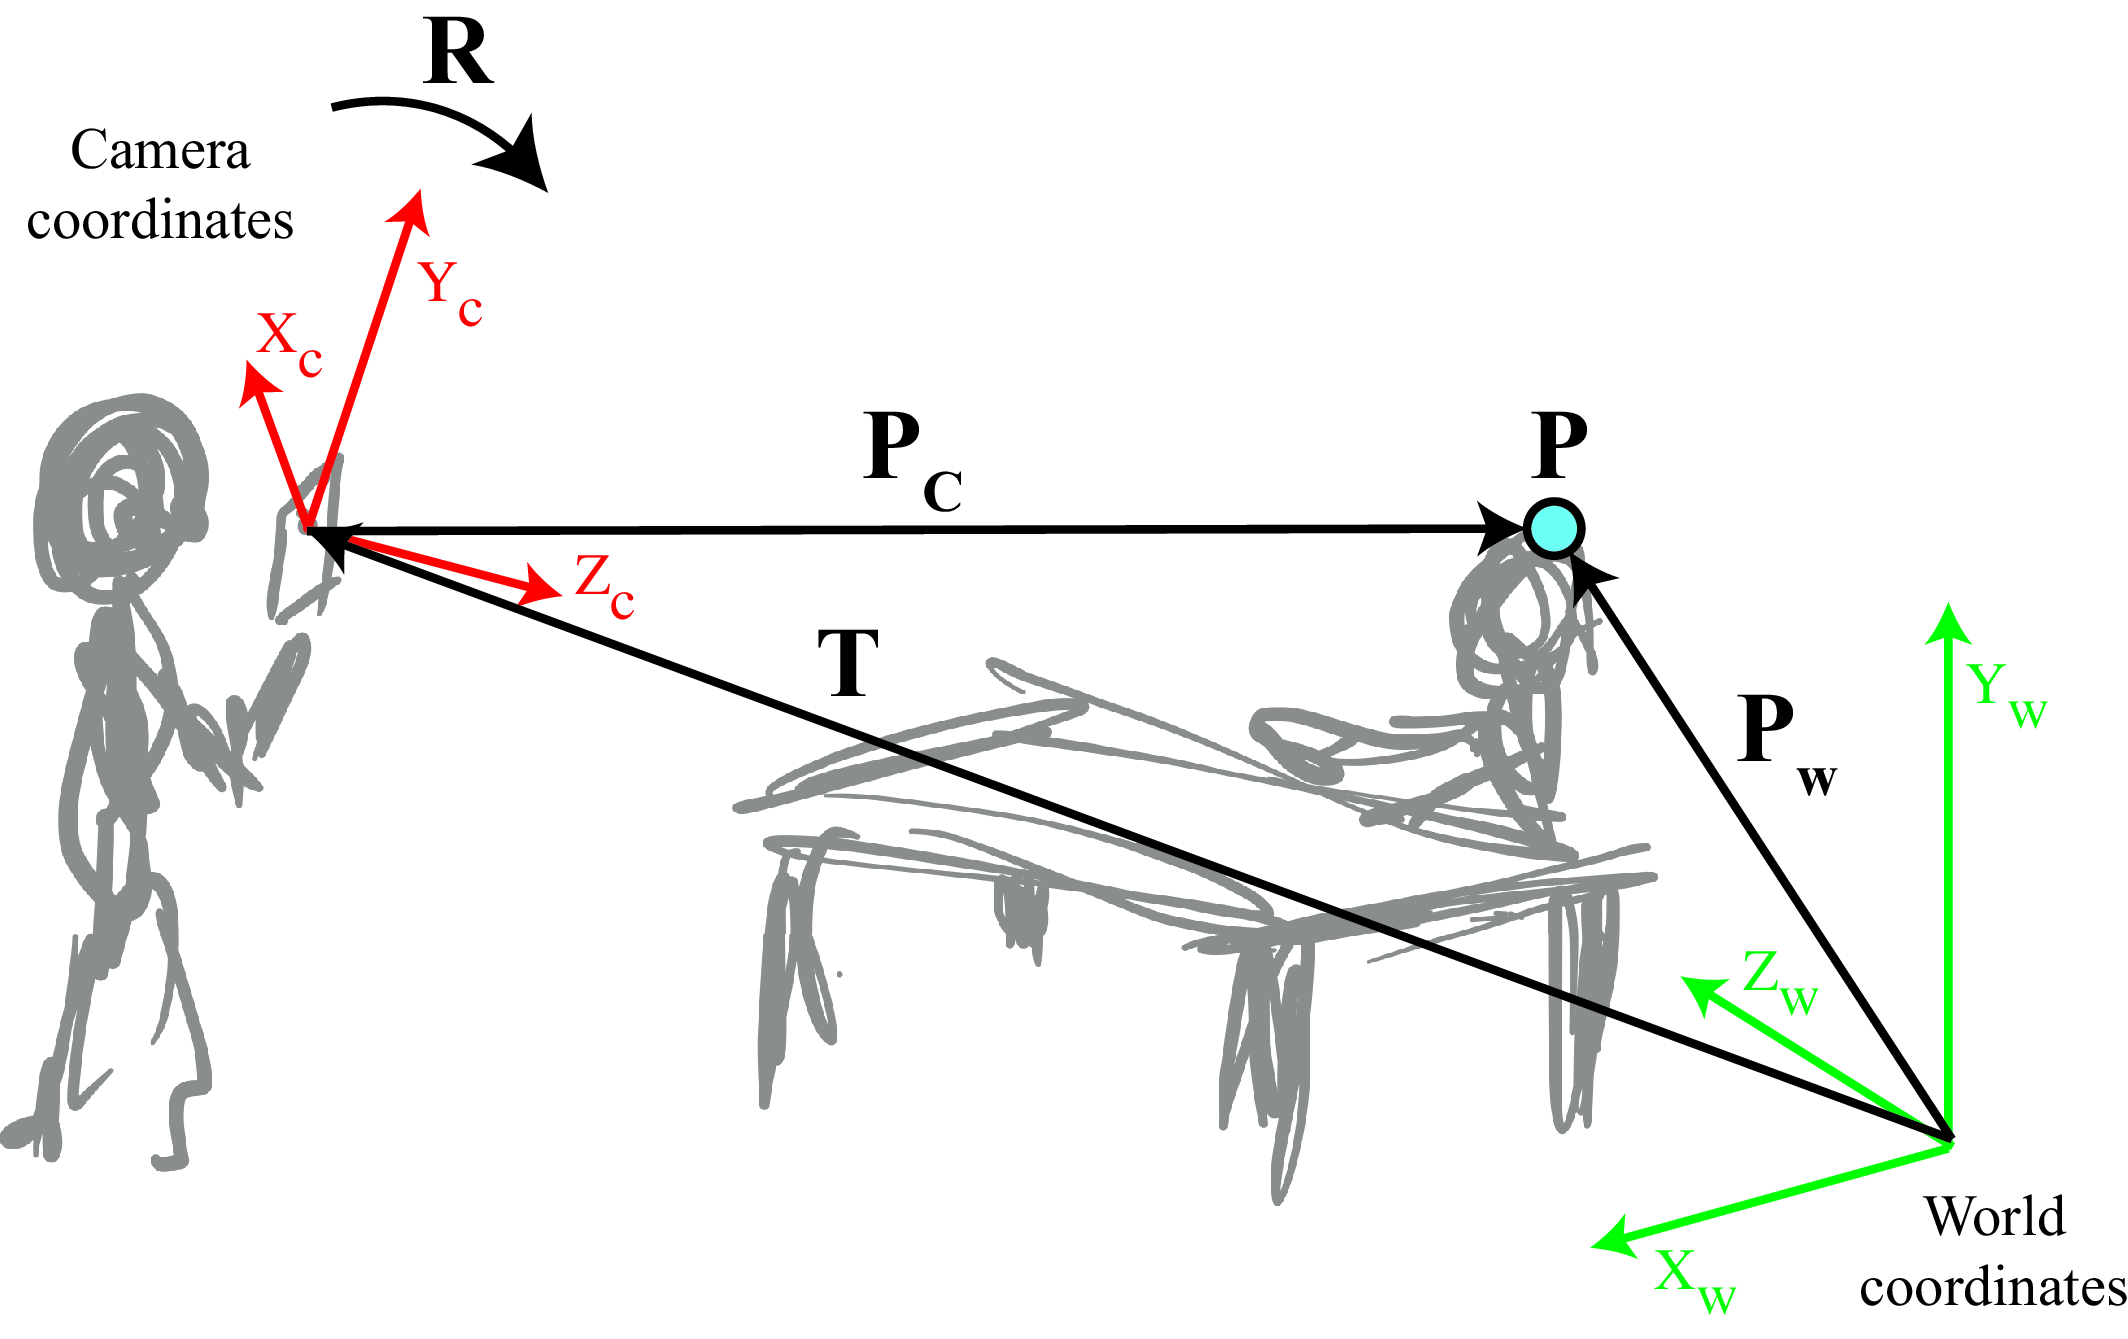
\includegraphics[width=0.5\textwidth]{imagenes/chapter2/world_and_camera_coordinates}
\end{center}
\caption{Visualización de las transformaciones necesarias, $[R|t]$, para transformar las coordenadas 3D a 2D, sacada de~\cite{VisionBookMIT}.}
\label{fig:WorldToImageCoordinates}
\end{figure}

\begin{equation}\label{eq:KMatrix}
    K = \begin{bmatrix}
        f & q_x & cx &\\
        q_y & f & cy &\\
        0 & 0 & 1 &\\
    \end{bmatrix}
\end{equation}
Donde $f$ es la distancia focal, $(q_x, q_y)$ son distorsiones de inclinación y $(c_x, c_y)$ es la correspondencia al punto principal (central) del sensor de la imagen.
Los parámetros $f$ y $c$ se pueden estimar a partir las características de las cámaras, si se conoce dicha información, o mediante 
métodos de calibración. Con la Figura~\ref{fig:ImageSensor} se observa que la posición de los píxeles escala 
con la distancia focal, $f$, de forma que se utiliza una constante $a$ en su lugar con la relación física con 
la cámara dada por la Ecuación~\ref{eq:EstimateAlpha}.
\begin{equation}\label{eq:EstimateAlpha}
    a = f\frac{N}{w}
\end{equation}
Donde $N$ es la longitud de la imagen en píxeles y $w$ es la longitud del sensor de la cámara.
No obstante, en caso de no poseer información al respecto del sensor se puede utilizar patrones de imágenes conocidas,
como un tablero de ajedrez, para estimar-los.
Finalmente, hasta el momento no se ha introducido ningún parámetro de distorsión al modelo de cámara. Sin embargo, 
existen diferentes distorsiones que pueden ocurrir como inclinación o distorsiones radiales. Estos son parámetros
adicionales que deben estimarse para obtener una re-proyección precisa.
\begin{figure}[htp]
\begin{center}
    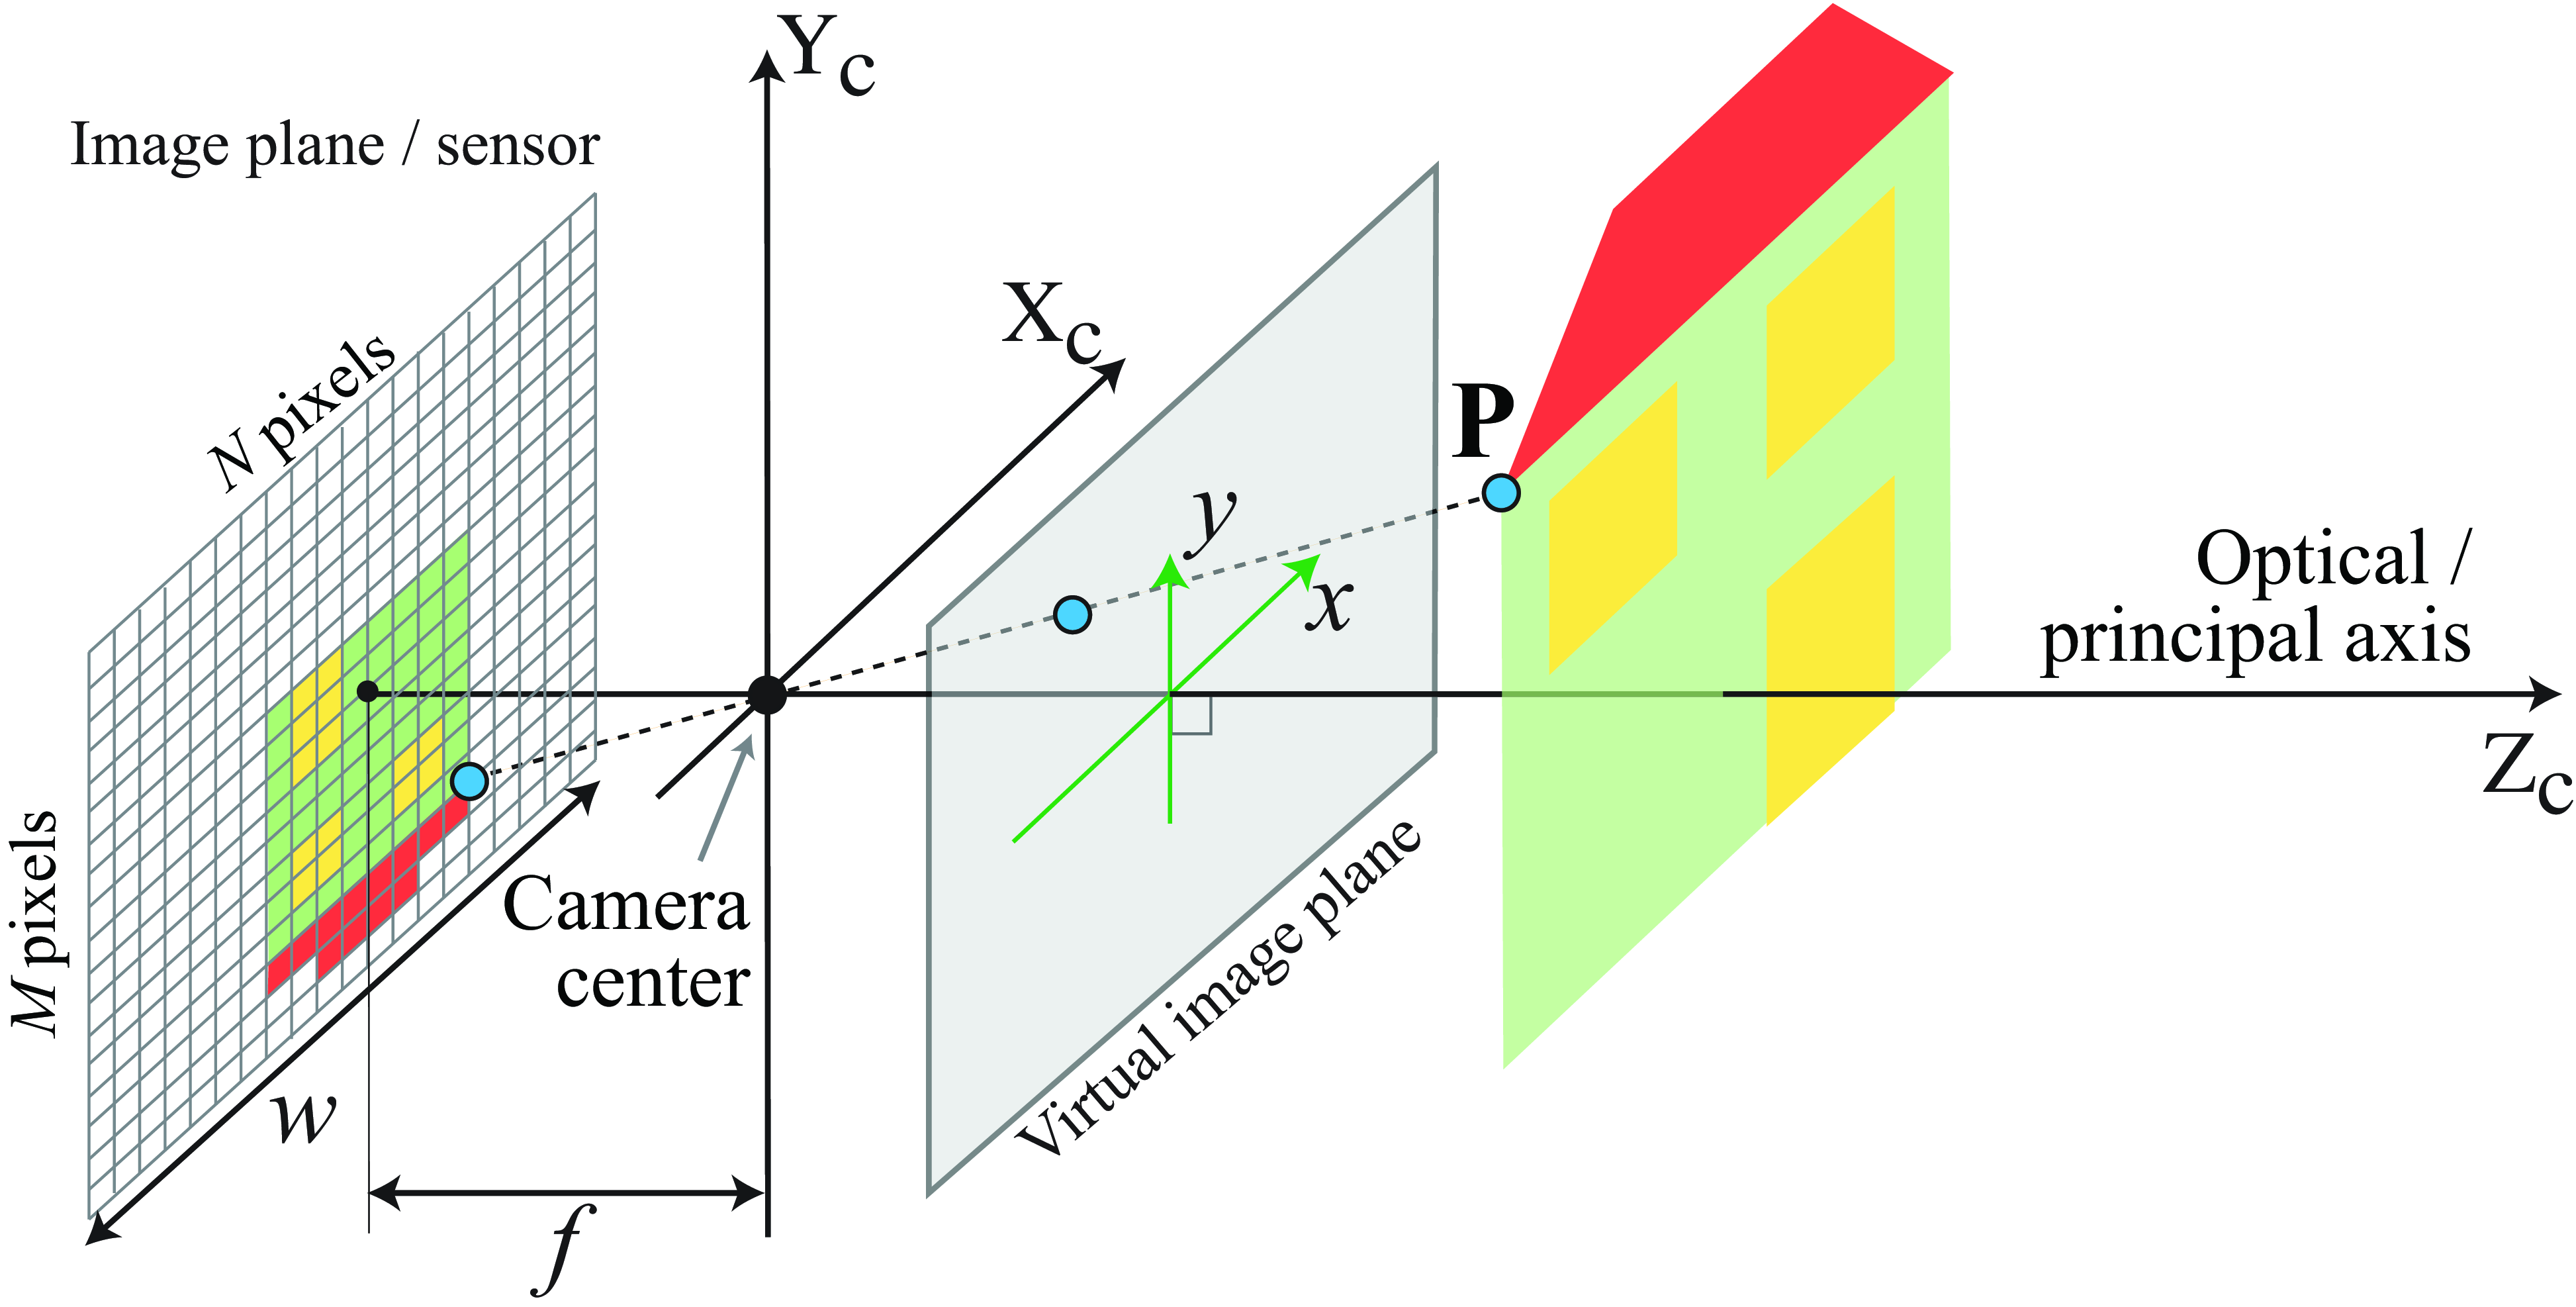
\includegraphics[width=0.5\textwidth]{imagenes/chapter2/pinhole_and_sensor}
\end{center}
\caption{Proyección de una imagen sobre el sensor de una cámara~\cite{VisionBookMIT}.}
\label{fig:ImageSensor}
\end{figure}
\section{Metrología de vista única}
La metrología de vista única (SVM) se refiere al conjunto de técnicas y principios que permite la extracción 
de información geométrica del espacio 3D a partir de una única imagen 2D, habitualmente captura por una 
cámara de perspectiva. En contra de los métodos tradicionales de fotometría o métodos multivista que
dependen de vistas calibradas para triangular la profundidad, SVM tiene la restricción de utilizar solamente 
una imagen y, aún así, obtener la escala absoluta de los objetos detectados~\cite{SVMIW}.
\par 
Es un problema realmente desafiante dada la pérdida de información de profundidad en proceso de obtención 
de la imagen. Al proyectar una escena 3D sobre el plano de imagen 2D, se colapsan los distintos puntos de 
profundidad sobre la misma coordenada de píxel. Como resultado, múltiples configuraciones de la escena 3D 
pueden resultar en la misma imagen, haciendo que el proceso inverso, de obtener información 3D a partir de 
la imagen 2D, sea realmente costoso sin suposiciones adicionales.
\par
Es por ello, que los métodos de SVM se basan en principios de geometría proyectiva, utilizando información
sobre los puntos de fuga, ortogonalidad, paralelismo y otras informaciones de la escena con fin de obtener 
los parámetros intrínsecos y extrínsecos de la cámara. Los primeros refieren a la distancia focal, tamaño 
del sensor y otros factores de la cámara, mientras que los segundos se refieren a su posición en el mundo, 
como la altura y la distancia al objeto de referencia. La premisa subyaciente de los métodos SVM es que,
aunque generalmente se pierden información de profundidad, existen invariantes geométricas que se preservan y
nos permiten razonar sobre la estructura y la escala~\cite{VisionBookMIT,Hartley2004}(véase las Figuras~\ref{fig:PalmaHorizon} y~\ref{fig:OfficeMeasurements}).
\par 
\begin{figure}[htp]
\begin{center}
    \subfloat{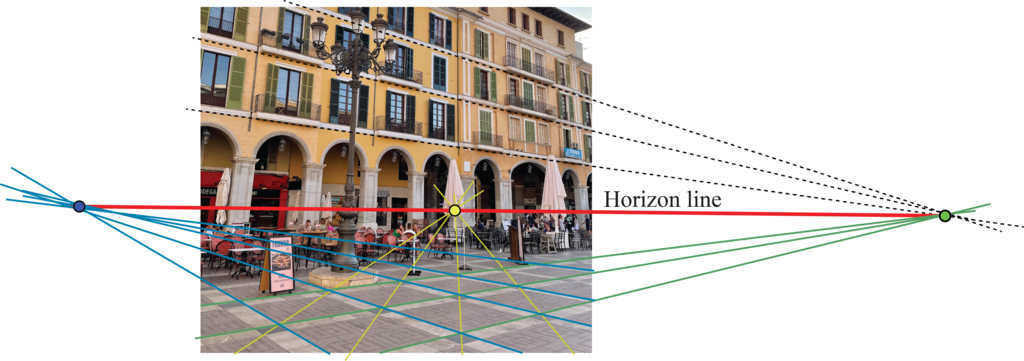
\includegraphics[width=0.6\textwidth]{imagenes/chapter2/palma_horizon}}
    \subfloat{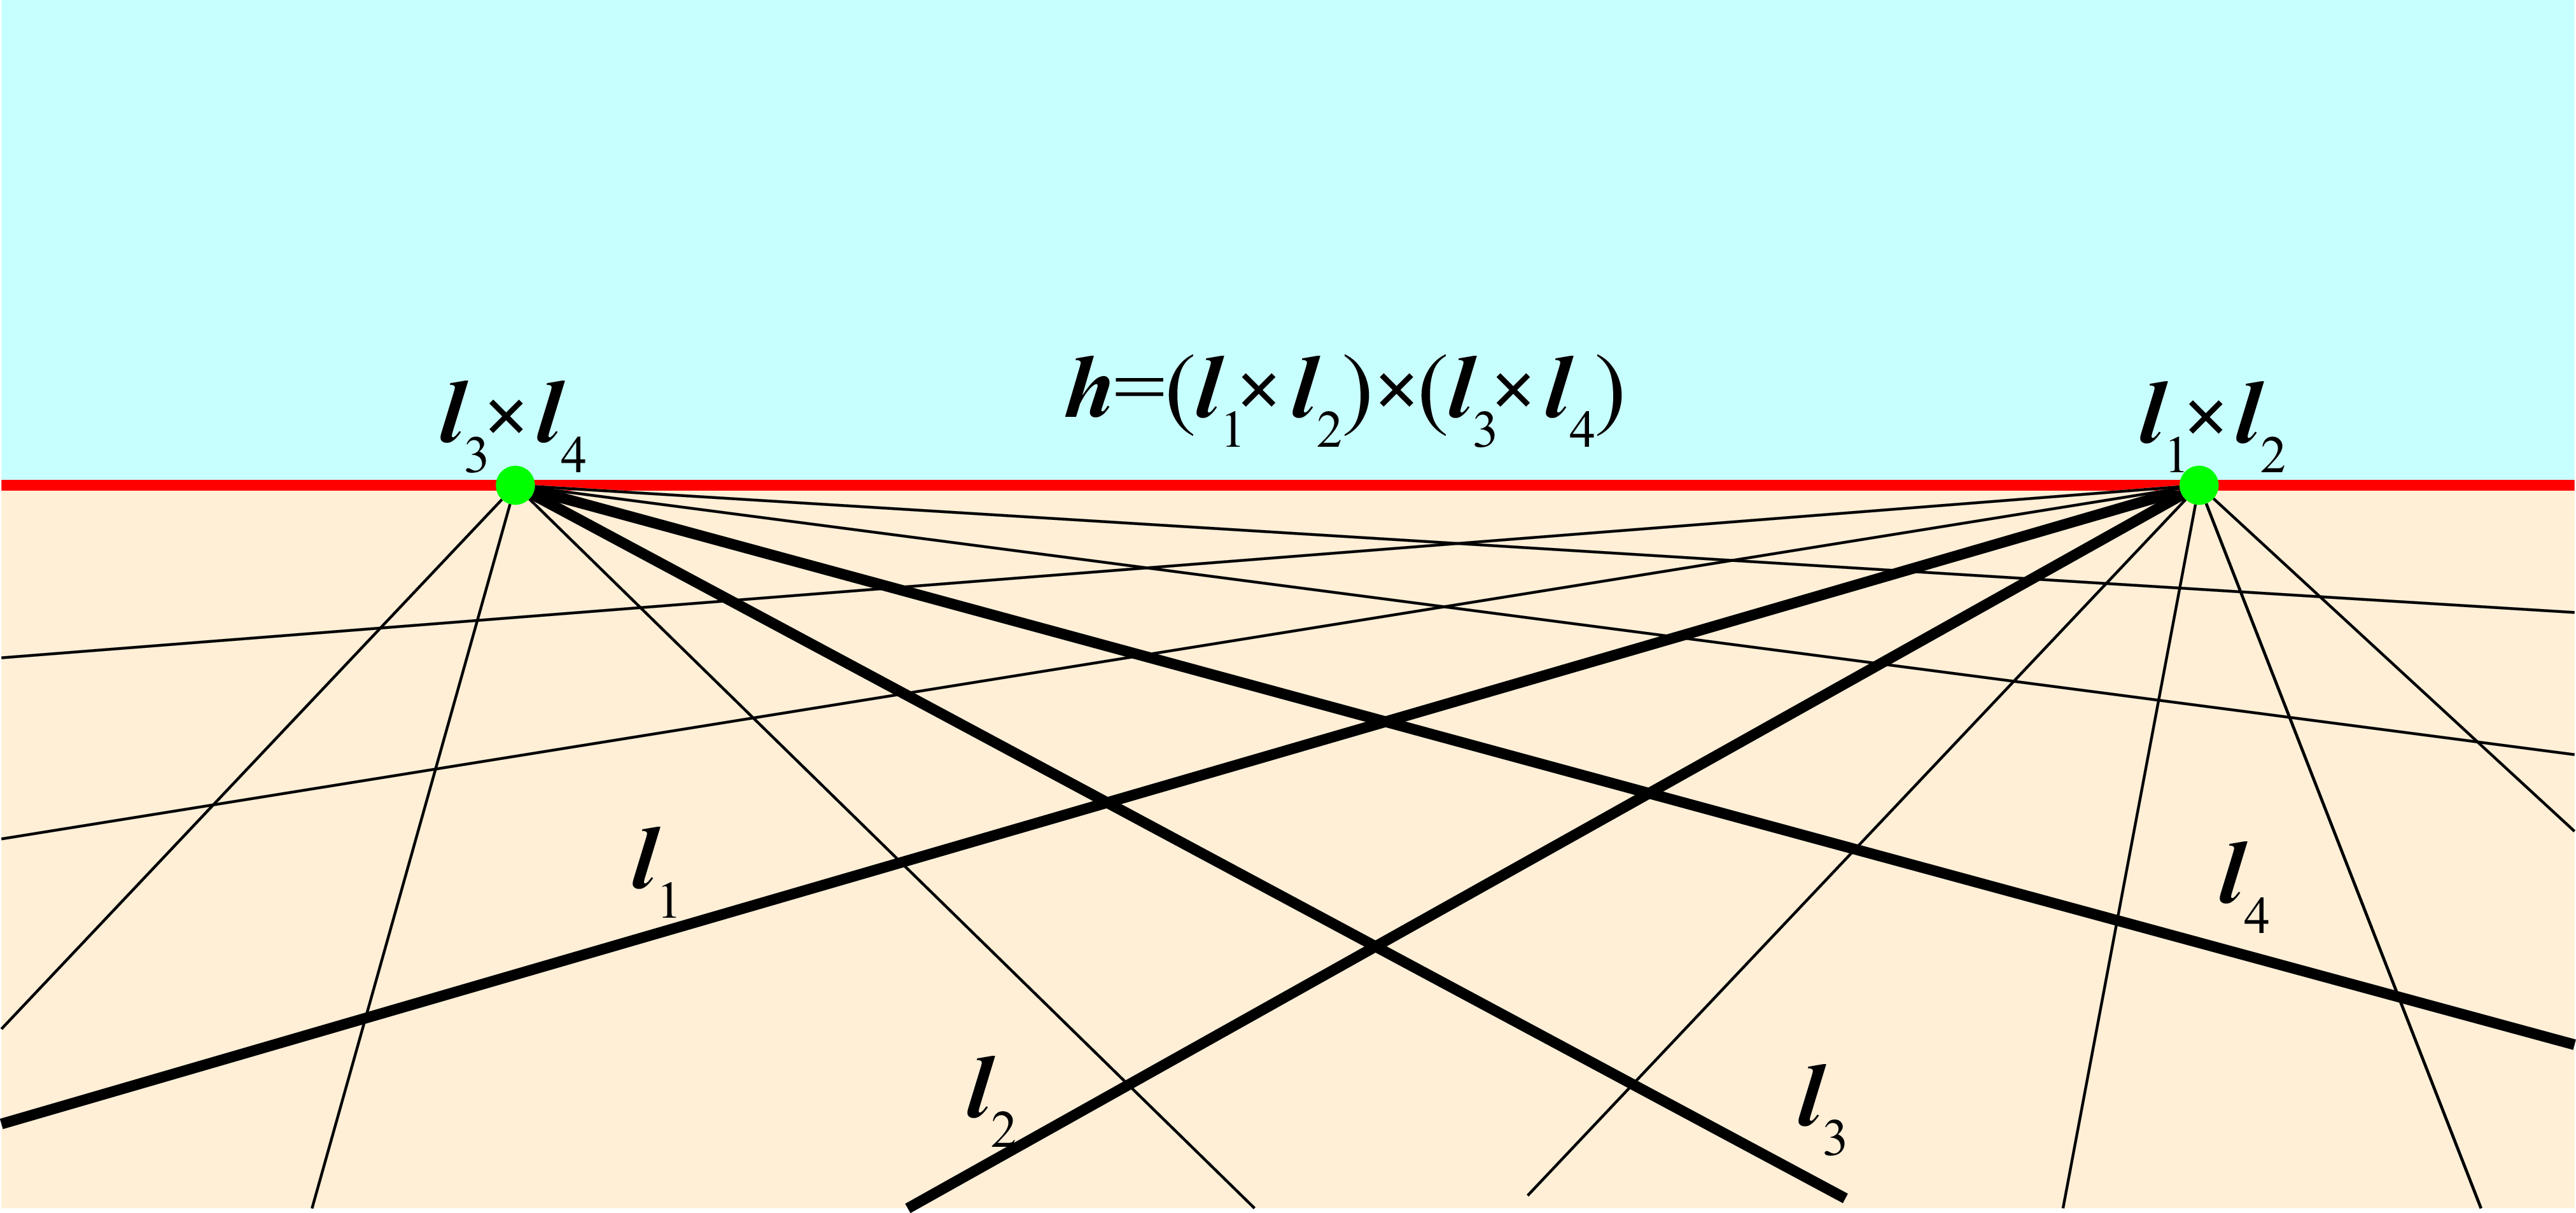
\includegraphics[width=0.4\textwidth]{imagenes/chapter2/horizon_line}}
\end{center}
\caption{Se observa como todas las líneas paralelas convergen a los mismos puntos de fuga.
Con dicha premisa geométrica, 
la línea del horizonte se puede calcular como se indica en la imagen a la derecha, como la intersección de cuatro líneas, paralelas dos a dos.
Imágenes extraídas de~\cite{VisionBookMIT}.
}
\label{fig:PalmaHorizon}
\end{figure}

Algunas de esas invariantes podrían ser dimensiones conocidas o restricciones geométricas (paralelismo u ortogonalidad de paredes y pisos).
Otro desafío inherente son los efectos de los errores en el modelo de cámara, distorsiones ópticas o supuestos de perspectiva inadecuados.
Estos factores pueden introducir desviaciones significativas en las estimaciones.
\par 
En los últimos años, se ha observado una integración creciente de métodos de aprendizaje profundo en la metrología de vista única. 
Las redes neuronales, entrenadas con grandes volúmenes de datos, han aprendido a capturar ``priors'' geométricos que permiten 
estimar automáticamente la escala y profundidad de los objetos a partir de una sola imagen. La combinación del enfoque 
impulsado por datos con fundamentos geométricas de metrología de vista única nos permite obtener mediciones fundamentadas y explicables.

\begin{figure}[htp]
\begin{center}
    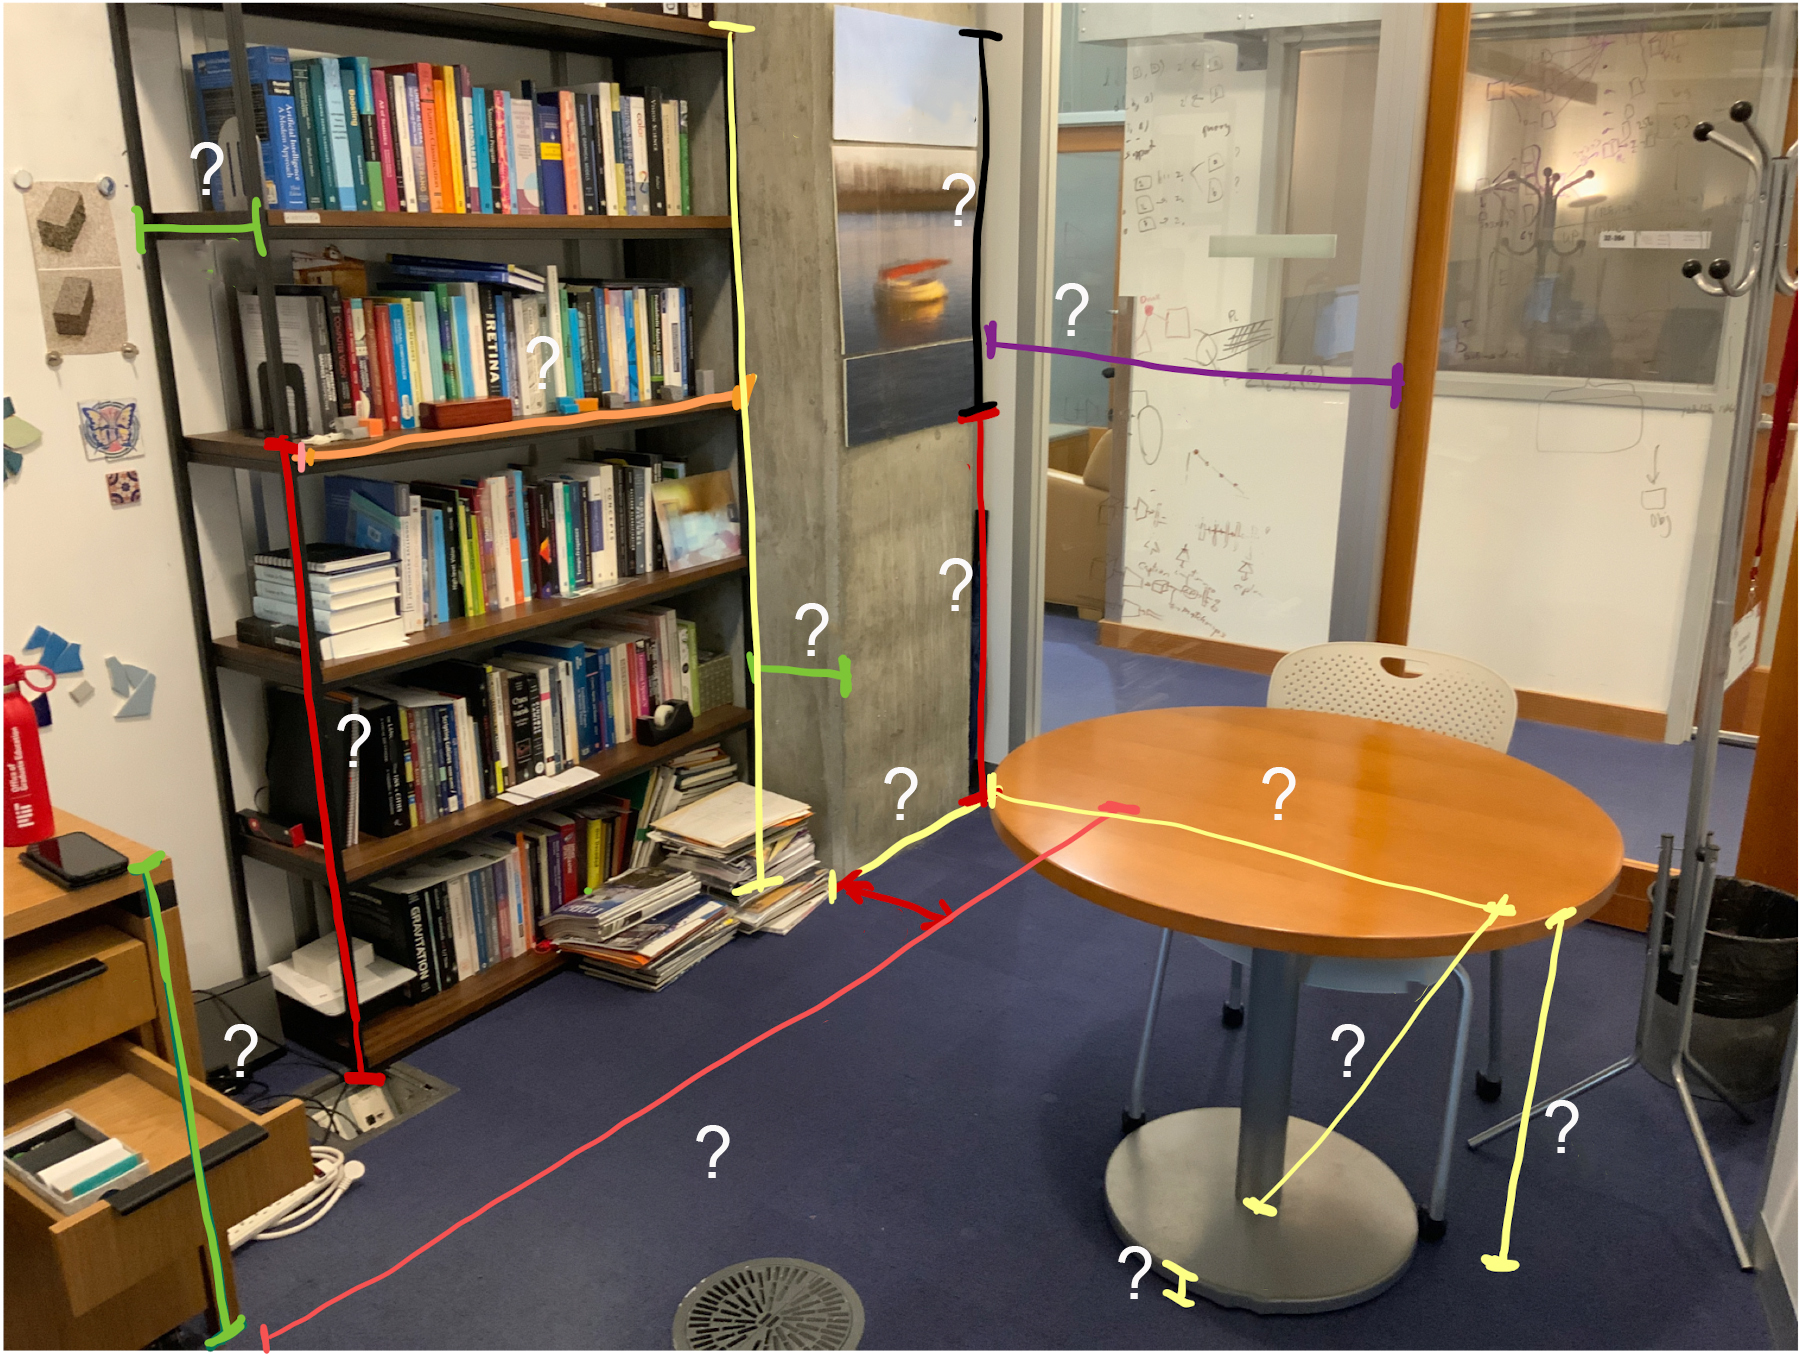
\includegraphics[width=0.5\textwidth]{imagenes/chapter2/office-measurements}
\end{center}
\caption{Ejemplo visual de información extraíble a partir una sola imagen si se conoce la longitud de alguna de líneas, extraída de~\cite{VisionBookMIT}.
}
\label{fig:OfficeMeasurements}
\end{figure}

\section{Aprendizaje automático y profundo}
El aprendizaje automático~\cite{IAModernApproach} es una rama del campo de la inteligencia artificial, 
cuyo objetivo principal es dotar a las máquinas de la capacidad de aprender a partir de los datos sin ser explícitamente
programadas para ello. El aprendizaje automático permite extraer patrones y realizar predicciones en base a los datos por 
medio de algoritmos y modelos estadísticos~\cite{LearningFromData}. Esta capacidad resulta especialmente valiosa para 
problemas complejos, difíciles de definir, que no tengan una solución analítica directa o en los que obtenerla resulte computacionalmente costoso.
\par 
Dentro del ámbito del aprendizaje automático (DL, por sus siglas en inglés), ha cobrado gran relevancia el aprendizaje profundo, 
que a diferencia de los modelos anteriores donde tenemos un conjunto de variables 
extraídas por un humano experto, las características sobre la cual inferimos 
son obtenidas por el propio modelo automáticamente~\cite{DeepLMITPress, DeepLearningNature, DeepLearningInNN}.
Los modelos de aprendizaje profundo están fuertemente inspirados en la estructura y funcionamiento del cerebro humano (véase la Figura~\ref{fig:ANNVisualization}). 
En términos generales, la extracción automática de características suele 
desempeñar mejores resultados frente a las características extraídas manualmente.
\par
\begin{figure}[htp]
  \centering
  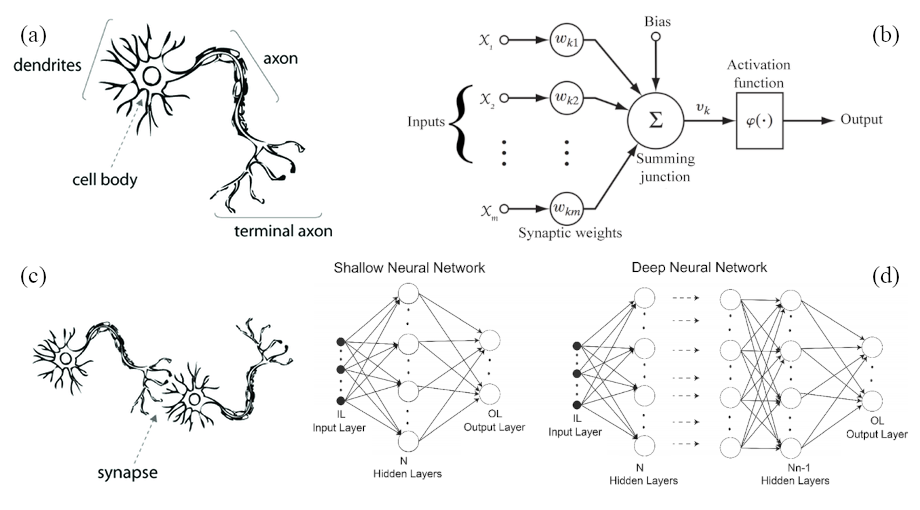
\includegraphics[width=0.7\textwidth]{imagenes/chapter2/ANNVisualization.png}
  \caption[Ejemplo gráfico de una red neuronal.]
  {Ejemplo gráfico de una red neuronal~\cite{NeuronImages, NeuronSimilarity,ShallowAndDeepNN}. 
    (a) y (b) muestran una neurona biológica y una artificial, respectivamente. 
    (c) describe el proceso mediante el cual las neurones se comunican entre sí para transmitir información (sinapsis). 
    (d) muestra dos redes neuronales artificiales: 
    a la izquierda, una red neuronal superficial (\emph{shallow}), con una única 
    capa oculta; a la derecha, una red neuronal profunda (\emph{deep}), con múltiples capas ocultas.
  }
  \label{fig:ANNVisualization}
\end{figure}
En particular, las redes neuronales artificiales (ANN, por sus siglas en inglés) simulan de forma abstracta el comportamiento 
de las neuronas biológicas~\cite{ANNForPattern, ANNCambridge}. Estas redes constan de una serie de capas: una capa de entrada, 
una o varias capas ocultas y una capa de salida. El proceso de aprendizaje en una red neuronal se puede dividir en tres etapas 
principales: entrada, procesamiento y salida. En la fase de entrada, los datos iniciales se introducen en la red. 
Durante el procesamiento, las distintas capas transforman progresivamente la información mediante combinaciones lineales (ponderadas) 
y funciones de activación no lineales, permitiendo así la construcción de representaciones internas cada vez más abstractas. 
Finalmente, en la etapa de salida, la red produce una predicción que se compara con el valor deseado. 
A partir de este error, calculado mediante una función de pérdida, se ajustan los pesos de la red a través de 
algoritmos de optimización, permitiendo la mejora continua.
\par

El aprendizaje de una red neuronal se logra mediante ese proceso iterativo, llamado entrenamiento.
Se repite el proceso descrito anteriormente varias veces con distintos ejemplos. El conjunto de datos es muy relevante para el correcto 
aprendizaje. Debe de ser representativo, extenso y limpio de anormalidades ya que estaremos extrayendo características 
y relevancias a partir de ellos. El desarrollo de estas técnicas ha supuesto un avance fundamental en múltiples campos, como la 
visión por computador. Permitiendo mejorar la detección de objetos, estimaciones de profundidad y metrología.
\section{Detección de objetos}
La detección de objetos es una de las tareas fundamentales dentro del campo de la visión por computador. Consiste en identificar y localizar 
instancias de objetos de interés dentro de una imagen o secuencia de vídeo. A diferencia de la clasificación de imágenes, donde se 
asigna una etiqueta global a la imagen (por ejemplo, un 1 si la imagen posee un gato), la detección implica además la estimación de la posición
espacial de los objetos (indicar dónde en la imagen está el gato)~\cite{ObjectDetectionSurvey}.
\par
En las primeras etapas, los detectores tradicionales combinaban la extracción de características manuales como Viola-Jones o HOG con 
clasificadores estadísticos~\cite{ObjectDetectionSurvey}. Se utilizaba ventanas deslizantes, que extraían trozos de la imagen, para calcular 
características locales. A continuación, se utilizaban dichas características para clasificar la presencia de objetos por medio de un 
clasificador estadístico, que aprendía con ejemplos de imágenes etiquetadas durante su entrenamiento (véase la Figura~\ref{fig:SelectiveSearch}). 
Sin embargo, estos enfoques presentaban importantes limitaciones en precisión, velocidad y fiabilidad frente a datos no vistos.

\begin{figure}[htp]
\begin{center}
    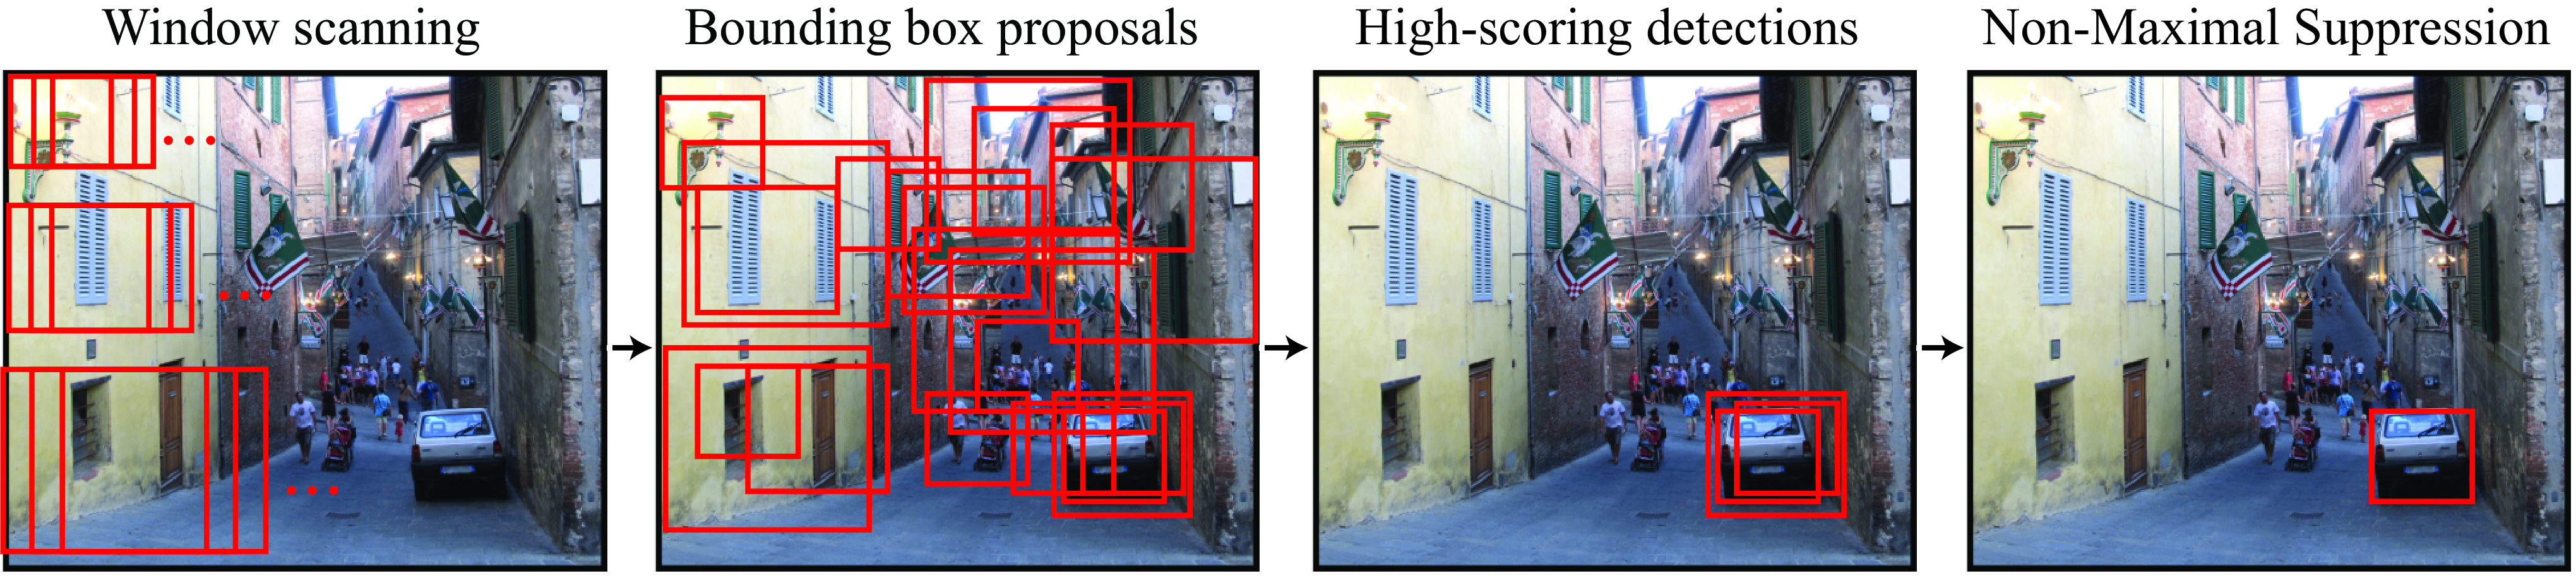
\includegraphics[width=0.7\textwidth]{imagenes/chapter2/selective_search}
\end{center}
\caption{
Visualización del proceso de ventana deslizante en busca de objetos~\cite{VisionBookMIT}, en este caso se busca un coche.
Se extraen características a múltiples escalas, se obtienen propuestas que se filtran en base al nivel de confianza del modelo. Finalmente, 
se ajusta la detección con métodos de refinamiento, como la eliminación de detecciones solapadas.
}
\label{fig:SelectiveSearch}
\end{figure}

\par 
La transición hacia modelos de aprendizaje más complejos ha sido impulsada por la disponibilidad de grandes conjuntos de datos anotados y 
por los avances en aprendizaje profundo~\cite{ObjectDetectionSurvey}. Sin embargo, muchos de los principios fundacionales siguen siendo 
los mismos: la combinación de representación visual, inferencia estadística y coherencia geométrica.

% %
\chapter{Estado del Arte}
\label{sec:EstadoDelArte}

% %
\chapter{Materiales y Métodos}
\section{Materiales}
Para la evaluación y validación de los métodos de metrología de vista única desarrollados en este trabajo,
se ha empleado un conjunto de datos privado, capturado específicamente con fines experimentales.
Dicho conjunto fue recogido en diversas localizaciones del entorno urbano mediante un sistema multicámara,
en el que se estableció como referencia principal una cámara con sensor de profundidad. A continuación,
se describen las cámaras utilizadas, así como su disposición relativa y características técnicas.
\subsection{Sistema de captura}
\begin{table}[htp]
\scriptsize
\centering
\begin{tabular}{lcccc}
\hline
\textbf{Cámara} & \textbf{Tipo} & \textbf{Focal (mm)} & \textbf{CMOS} \\
\hline
RealSense D455 (RS) & Profundidad & 1.93 &  1/4'' OV9782 \\
Tapo C120 (Cam1) & Tipo cajero & 3.17 &  1/2.9'' \\
Dahua IPC-HDBW2831 (Cam2) & Domo & 2.8 &  1/2.7'' \\
Hikvision DS-2CD2046 (Cam3) & Bullet & 2.8 &  1/3'' \\
\hline
\end{tabular}
\caption{Características técnicas de las cámaras utilizadas}
\label{tab:CaptureSystem}
\end{table}
En la Tabla~\ref{tab:CaptureSystem} se recogen las características técnicas de cada una de las cámaras.
Cada una de ellas se monta en su respectivo tripod. Se utiliza la cámara ``Intel RealSense D455'' (RS) como principal y
se calcula el posicionamiento de las demás en términos relativos (véase información adicional en el Apéndice~\ref{app:LocationConfig}).
Esto es debido a que se utilizará el sensor de profundidad, ``CMOS 1/4'' OV9782'', de la cámara RS para realizar los cálculos necesarios para estimar el
tamaño de los objetos en escena utilizando el método clásico. Las cámaras empiezan a grabar simúltaneamente, almacenando
la información tanto en memoria como a través de la red. Se obtienen grabaciones en cuatro ubicaciones diferentes: una sala de seminarios,
una rampa de entrada, un aparcamiento y una acera (véase la Figura~\ref{fig:DataExamples}).
\begin{figure}[htp]
\begin{center}
    \subfloat{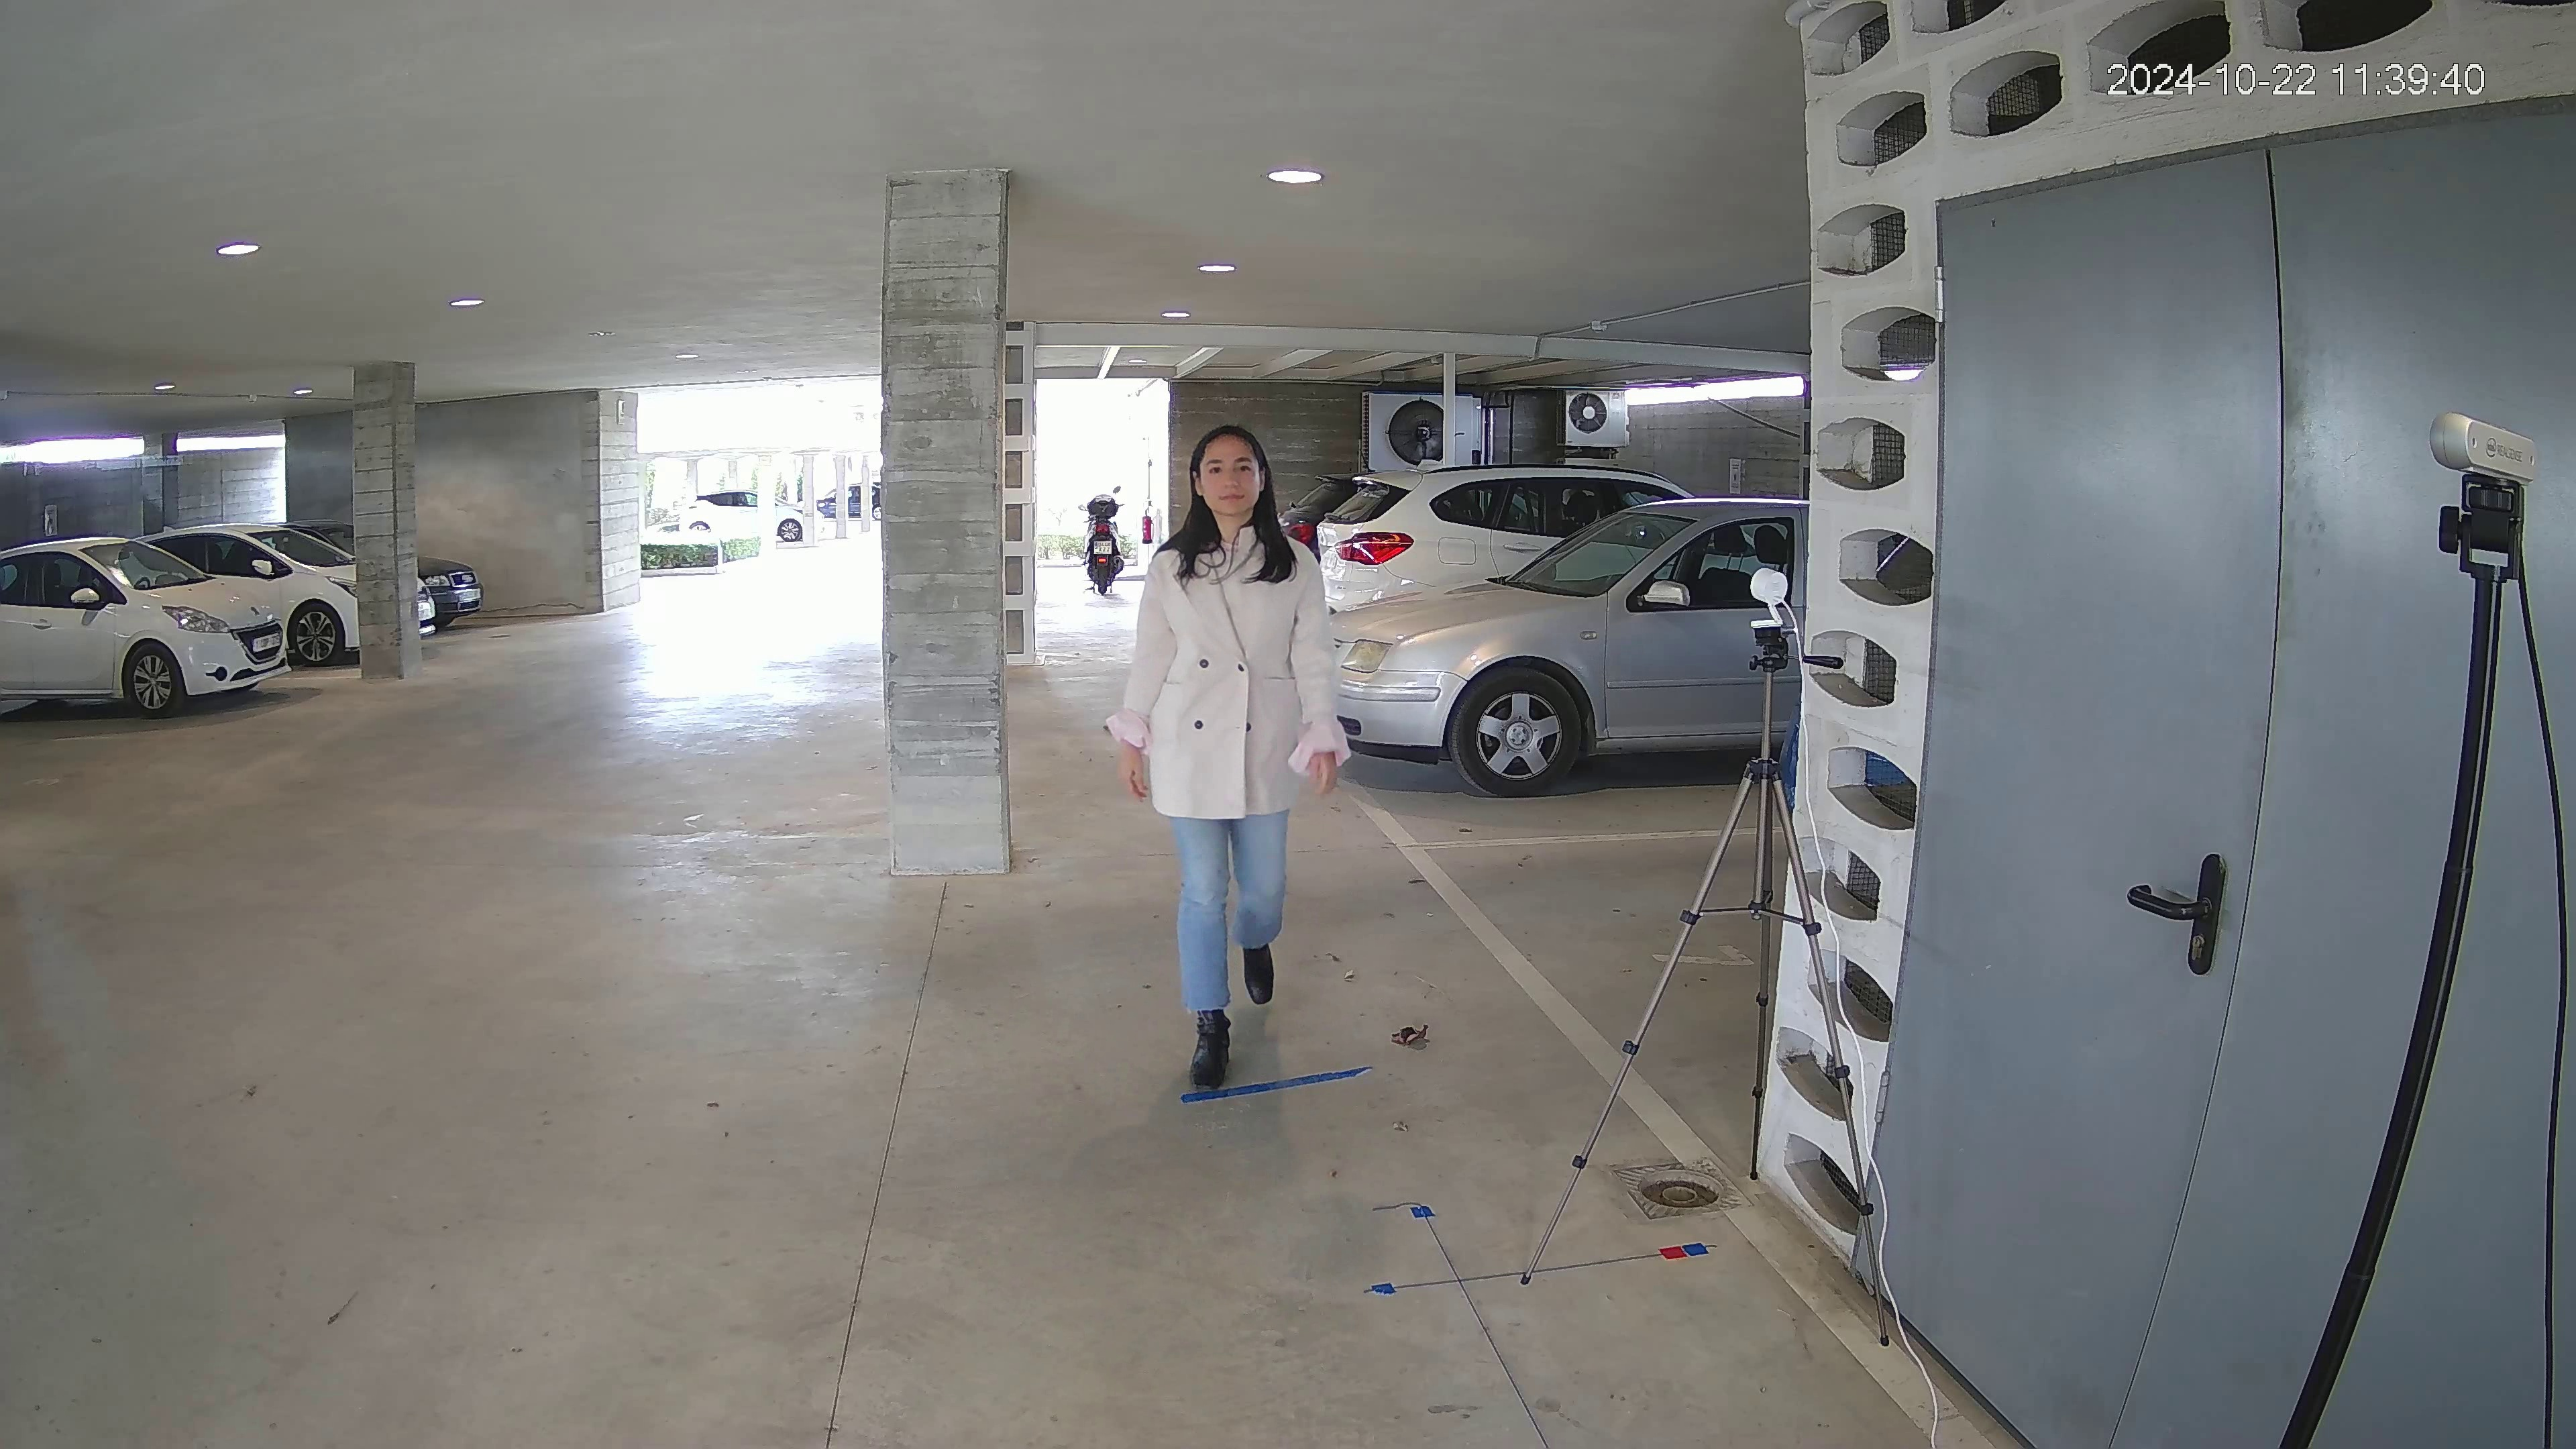
\includegraphics[width=0.5\textwidth]{imagenes/chapter4/ParkingLot}}
    \subfloat{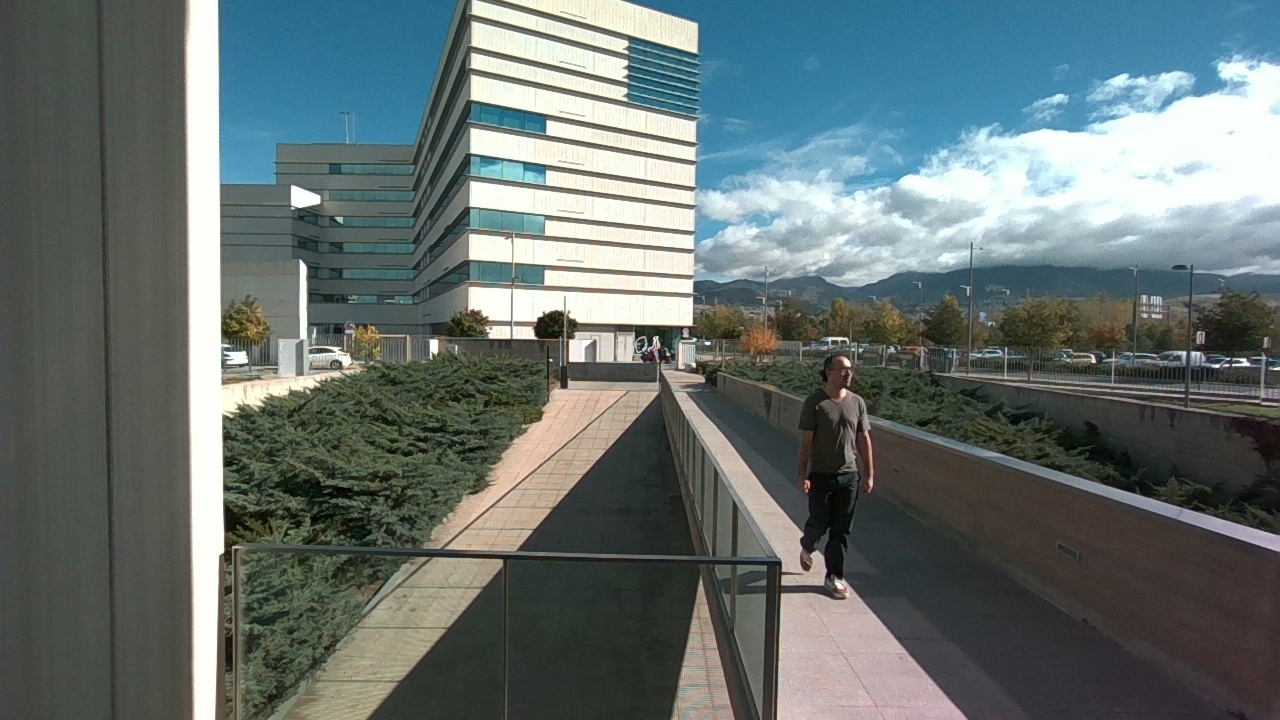
\includegraphics[width=0.5\textwidth]{imagenes/chapter4/EntranceRamp}}\\
    \subfloat{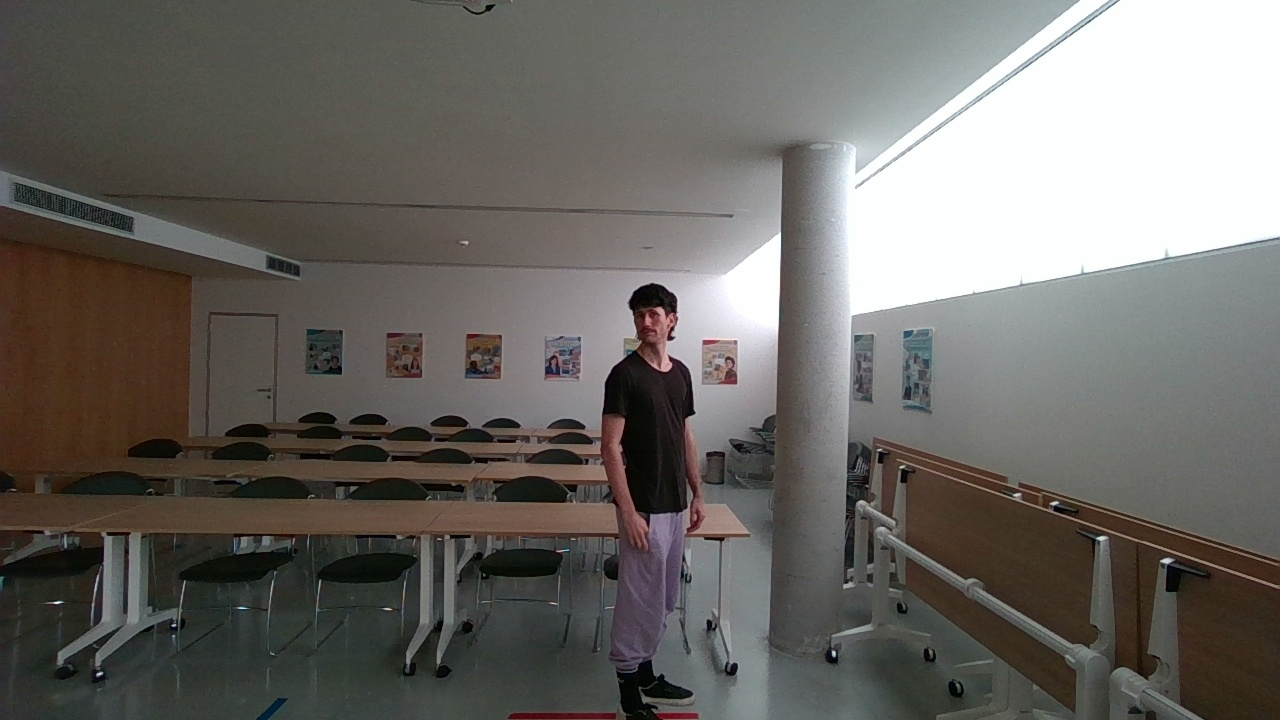
\includegraphics[width=0.5\textwidth]{imagenes/chapter4/SeminarRoom}}
    \subfloat{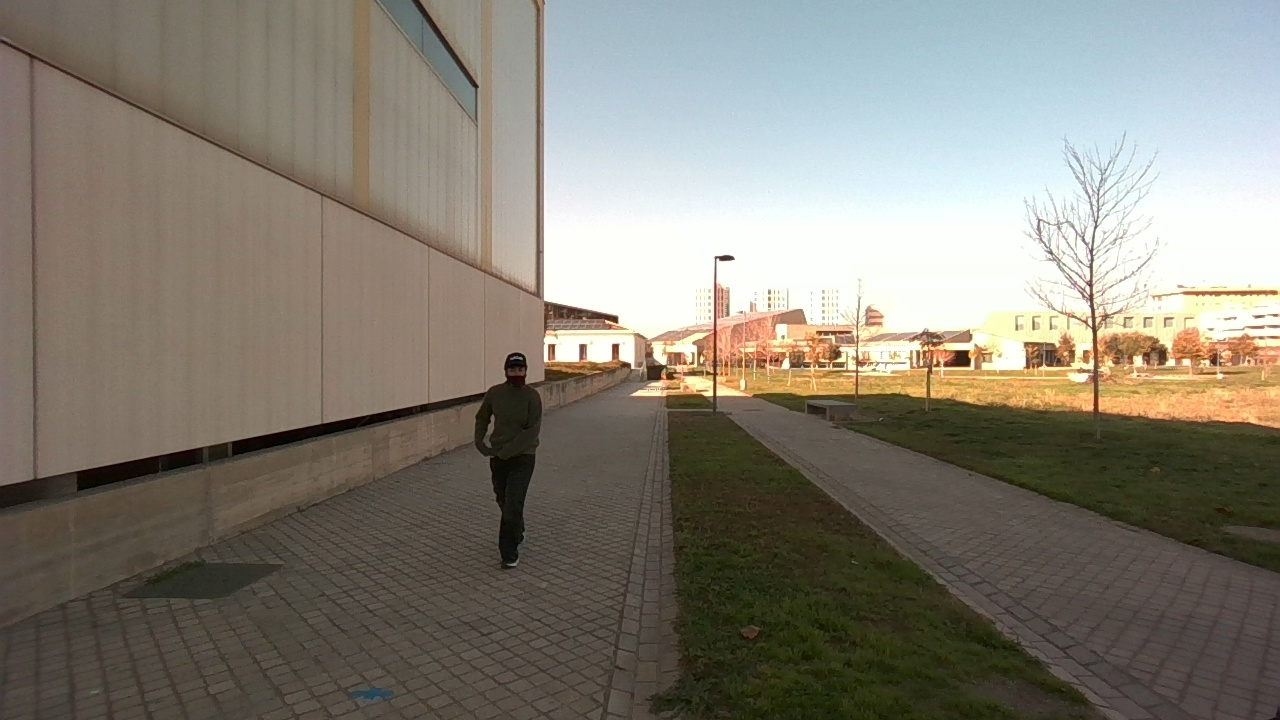
\includegraphics[width=0.5\textwidth]{imagenes/chapter4/Sidewalk}}
\end{center}
\caption{Ejemplo de grabaciones realizadas en las diferentes ubicaciones.}
\label{fig:DataExamples}
\end{figure}

% Nice end phrase perhaps?
Este conjunto de datos, capturado bajo condiciones reales y desde múltiples puntos de vista, ha permitido una evaluación robusta de
los métodos propuestos, facilitando el análisis de su rendimiento frente a diferentes configuraciones geométricas y
tipos de cámaras de vigilancia.
\subsection{Descripción de vídeos obtenidos}
\section{Métodos}
\subsection{Calibración utilizando información a priori}
\subsection{Calibración automática}

% %
\chapter{Implementación y Experimentos}
\section{Diseño experimental}
\subsection{Protocolo de validación experimental}
\subsection{Experimentos SVMIW}
\section{Discusión de resultados}

%
%\input{capitulos/06_Implementacion}
%
%\input{capitulos/07_Pruebas}
%
\chapter{Conclusiones y Trabajos Futuros}

%
%
\nocite{*}
% \bibliography{bibliografia/bibliografia}\addcontentsline{toc}{chapter}{Bibliografía}
% \bibliographystyle{unsrturl}
\newpage
\chapter{Bibliografía}
\printbibliography[heading=none, category=cited]
\appendix
\chapter{}
\section{Búsqueda en Scopus}
Se utiliza la siguiente combinación de búsqueda por terminología, palabras claves y conceptos relacionados con metrología de vista única:
\begin{lstlisting}[language=,basicstyle=\ttfamily\small,breaklines=true,frame=single,backgroundcolor=\color{gray!10}]
(TITLE-ABS-KEY("single view metrology" OR "single-view metrology" OR "single image 3D reconstruction" OR "monocular 3D reconstruction" OR "geometry from a single image" OR "single view geometry"))
AND (LIMIT-TO(SUBJAREA, "COMP") OR LIMIT-TO(SUBJAREA, "ENG"))
AND (LIMIT-TO(DOCTYPE, "ar") OR LIMIT-TO(DOCTYPE, "cp"))
\end{lstlisting}

\section{Configuración por Localización}\label{app:LocationConfig}
\begin{table}[htp]
\scriptsize
\centering
\begin{tabular}{lccc}
\hline
\textbf{Cámara} & \textbf{Altura (m)} & \textbf{Posición relativa a RS} \\
\hline
RS (RealSense) & 1.593 & (0, 0, 0) \\
Cam1 (Tapo C120) & 1.509 & (-0.4000, -0.0840, +0.4000) \\
Cam2 (Dahua) & -- & -- \\
Cam3 (Hikvision) & -- & -- \\
\hline
\end{tabular}
\caption{Sala de Seminarios}\label{tab:SeminarRoom}
\end{table}

\begin{table}[htp]
\centering
\scriptsize
\begin{tabular}{lccc}
\hline
\textbf{Cámara} & \textbf{Altura (m)} & \textbf{Posición relativa a RS} \\
\hline
RS (RealSense) & 1.555 & (0, 0, 0) \\
Cam1 (Tapo C120) & 1.332 & (+0.4510, -0.2230, +1.9280) \\
Cam2 (Dahua) & 1.498 & (-0.7630, -0.0570, +1.4980) \\
Cam3 (Hikvision) & -- & -- \\
\hline
\end{tabular}
\caption{Aparcamiento}\label{tab:ParkingLot}
\end{table}

\begin{table}[H]
\centering
\scriptsize
\begin{tabular}{lccc}
\hline
\textbf{Cámara} & \textbf{Altura (m)} & \textbf{Posición relativa a RS} \\
\hline
RS (RealSense) & 1.530 & (0, 0, 0) \\
Cam1 (Tapo C120) & 1.350 & (-0.6260, -0.1800, +0.2640) \\
Cam2 (Dahua) & 1.790 & (-0.4250, +0.2600, -0.1200) \\
Cam3 (Hikvision) & 2.250 & (-0.7100, +0.7200, -0.5950) \\
\hline
\end{tabular}
\caption{Acera}\label{tab:Sidewalk}
\end{table}

\begin{table}[H]
\centering
\scriptsize
\begin{tabular}{lccc}
\hline
\textbf{Cámara} & \textbf{Altura (m)} & \textbf{Posición relativa a RS} \\
\hline
RS (RealSense) & 1.810 & (0, 0, 0) \\
Cam1 (Tapo C120) & -- & -- \\
Cam2 (Dahua) & -- & -- \\
Cam3 (Hikvision) [idai10] & 2.050 & (-1.2130, +0.2400, 0) \\
Cam3 (Hikvision) & 2.050 & (-1.2130, +0.2400, +0.6120) \\
\hline
\end{tabular}
\caption{Rampa de Entrada. Hay un posicionamiento distinto para la cámara 3, para 1 sujeto específico (idai10).}\label{tab:EntranceRamp}
\end{table}


\thispagestyle{empty}
%%\input{apendices/paper/paper}
%\input{glosario/entradas_glosario}
% \addcontentsline{toc}{chapter}{Glosario}
% \printglossary
%\chapter*{}
%\thispagestyle{empty}
\end{document}
